This chapter is aimed at comparing Lava and ForSyDe, two DSLs (\textit{Domain
  Specific Languages}) embedded in Haskell.  The comparison was made at the
initial stage of the thesis, as a means of acquiring a picture of the previous
work in the Functional Programming and Hardware Description field, in order to
hopefully reuse earlier design techniques and to provide ForSyDe's compiler
with state-of-the-art features. Thus, at the time of writing this comparison
the compiler was not yet designed.


  During the comparison, the reader will get familiar with the
  important concept of \textit{Embedded Compiler}. Furthermore, by the end
  of the chapter he (or she) will ...  

  \begin{itemize}
  \item  ... be able to understand the problems
    related to represent circuits in a purely functional programming
    language such as Haskell.
  \item ... hopefully have acquired a valuable background
    in the Hardware design and Functional Languages field along with
    an up-to-date view of the previous work related to this thesis.
  \end{itemize}

  \section{Introduction}
  The complexity of electronic designs has tremendously risen during the past
  two decades which, together with the Industry's exigency of extremely
  short time-to-market periods have made RTL-level tools no longer fit
  nowadays circuit design requirements. Thus, there has been a
  natural move to a higher level of abstraction known as
  \textit{System Level Design}.

  The two most commonly-used RTL-level HDLs (Verilog and VHDL) are far
  too verbose and concrete to cleanly give a general view of a
  complex system.

  Therefore, new languages are needed to provide a solution for the
  aforementioned problems.  Among other approaches which require
  creating a new programming language from scratch, the
  \textit{Embedded Approach} saves the designer having to learn a new
  syntax and makes possible to reuse all the existing tools (i.e.
  compilers, interpreters ...)  surrounding the \textit{host
    language}.

  Furthermore, the expressiveness of declarative languages such as
  Haskell seems to suit the abstraction level of \textit{System Level
    Design}  \cite{declarative} and hardware design semantics
   \cite{funhw}.

  During the rest of this chapter, two Haskell-embedded language
  approaches will be compared: Lava \cite{lava} and
  ForSyDe \cite{forsyde}. The later targets synchronous systems in
  general (that is, systems in which a single global clock is
  used\footnotemark \footnotetext{ForSyDe supports as well a
    \textit{multi-rate model} by using \textit{multi-rate interfaces},
    able to connect different synchronous sub-domains working at
    different clock rates.}), while the first specifically describes
  synchronous hardware (a concrete type of synchronous system after
  all) and is the most mature of the two.
  
\section{Design flow}
Lava and ForSyDe were independently developed by the Swedish
universities of Chalmers and KTH.

Figures \ref{fig:lava} and \ref{fig:forsyde} contain diagrams
describing the simplified design flow to be followed when modelling with
Lava and ForSyDe.  As it will be later seen, the flow is quite
similar to the traditional compilation model of a
general-purpose programming language.

It is easy to suspect that both Lava and ForSyDe follow a similar
approach, sequentially divided in two stages:


\begin{enumerate}[1)]
  \item The designer models a circuit in Haskell, making use
    of the Lava or ForSyDe libraries.



  \item The obtained model is automatically processed by a compiler in
    order to attain different \textit{goals}: simulation, testing,
    verification and translation to a less abstract HDL (e.g. VHDL)
    directly synthesizable to hardware. The different flavours of this
    stage are known as \textit{Interpretations} in Lava and
    \textit{Implementation Mappings} in ForSyde. In the rest of this
    chapter I will refer to them with the wider spread term:
    \textit{backends}.  The details of these backends will be
    described in next section.


\begin{landscape}
  \begin{figure}
    \centering
    \begin{minipage}[t]{.45\linewidth}
      \caption{Lava's design flow}\label{fig:lava}
      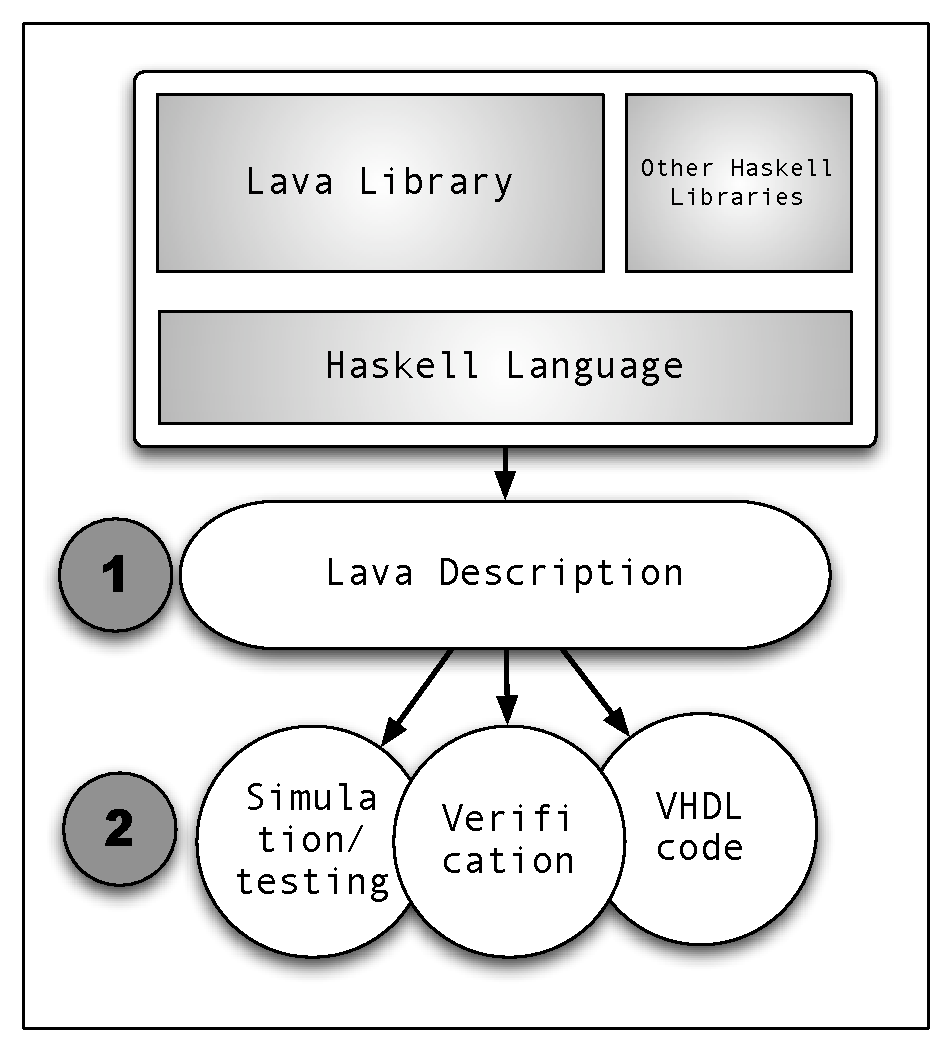
\includegraphics[width=\linewidth]{Lava.pdf}
    \end{minipage}
    \hfil
    \begin{minipage}[t]{.45\linewidth}
      \centering
      \caption{ForSyDe's design flow}\label{fig:forsyde}
      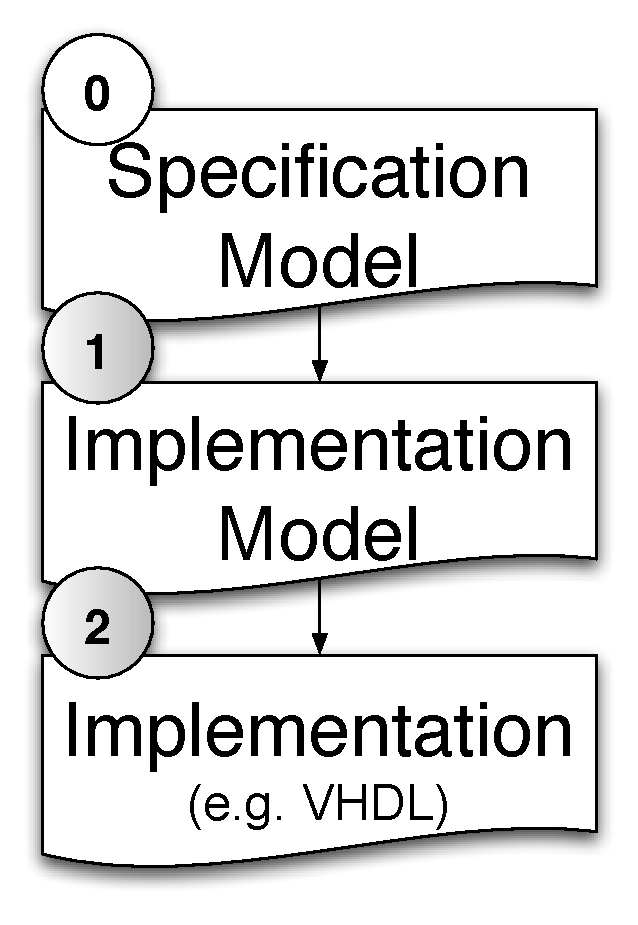
\includegraphics[width=\linewidth]{ForSyDe.pdf}
    \end{minipage}
  \end{figure}
\end{landscape}


    This stage slightly differs depending on the language used, being more
    complex, and potentially more likely to include optimizations in
    the case of ForSyDe, due to the application of \textit{Design
      Transformations}.
    
    ForSyDe has a strong formal base which allows the designer to work
    at a highly abstract functional level. The abstraction level is
    lowered\footnote{ForSyDe currently lacks an automatic tool
      for this purpose and transformations need to be applied
      manually. Either the case,  \cite{forsyde:thesis} proves it would not
      only feasible but quite straight-forward to implement.} by
    applying \textit{Transformation Rules} to the provided hardware
    descriptions. That is captured in figure \ref{fig:forsyde} as the
    transition from 2a to 2b.

    The internal details of  ForSyDe's \textit{Refinement} are out of
    the scope of this chapter but is worth to mention that the
    \textit{Transformation Rules} can be divided in \textit{semantic
      preserving} and \textit{design decisions}. The later ones
    change the semantics of the model and thus, its application must be
    supervised by the designer.
\end{enumerate}
\section{Backends}
As it was mentioned previously, Lava is in a more mature state than
ForSyDe, having a whole set of tools surrounding it.

On the other hand, ForSyDe only currently supports simulation by
direct execution of its Haskell models\footnote{\textit{Zero-delays},
  circuit feedback loops without delays, are forbidden in ForSyDe and
  thus cannot be simulated.}. Even with that, a \textit{template
  system}, in which every library function has a preassigned VHDL
template, has been already planed and a few prove-of-concept
examples \cite[Chapter 6]{forsyde:thesis} back it as a promising
approach.

As of the time of writing this thesis, Lava has three available backends:

\begin{itemize}
\item \textbf{Simulation and random testing}. A circuit simulation
  is carried out by interpreting each component of its
  structure\footnote{Zero-delays are only permitted when performing a
    \textit{constructive} simulation by using \texttt{simulateCon},
    see Lava's documentation \cite{lava:thesis} for details.}.

  In addition, Lava allows to test properties of a
  design on random data through a language which is highly inspired in
  \textsf{QuickCheck} \cite{quickcheck}.
  
  \textsf{QuickCheck} is as well embedded in Haskell and has been
  developed independently of the Lava system. That makes it suitable
  of being used for other purposes than testing circuit properties.
  Indeed, \textsf{QuickCheck} has been successfully employed in many
  other projects and could certainly be integrated into ForSyDe if
  desired.

\item \textbf{Verification}. Lava is able to generate a logical
  formula representing the circuit. That formula, along with
  properties defined by the designer, are given to an external theorem
  prover which can prove or disprove their validity.
  
  Despite how promising verification can seem at first sight, there is
  a well-known underlying theoretic limitation within First Order
  Logic which makes it semi-decidable\footnote{Any valid theorem can
    be proven but invalid clauses are not always identified.}.
  Furthermore, First Order Logic verification is computationally
  expensive (a NP-complete problem) and usually the prover has to be
  ``helped'' by splitting proves in smaller ones.
  
  Fortunately random testing is still at hand and, although it does
  not answer the validity question, it can be good enough in most of
  the cases.


  
  Nevertheless, theorem provers can give an answer about the validity
  of many circuit properties, being especially valuable in critical
  design parts\footnote{Intel designers surely regret not making
  extensive use of formal verification methods in an earlier stage.
  Famous bugs as the Pentium{\tiny $^{\textregistered}$}'s
  \texttt{F00f} \cite{f00f} and \texttt{FDIV} \cite{fdiv}, could
  probably have been avoided by applying formal methods. Nowadays
  Intel makes use of the \textit{Forte Verification
  Environment} \cite{forte}, currently based on
  \reFLect{ \cite{reflect}}, and formerly on FL \cite{fl}, two
  functional programming languages.}. As opposed to simulation and
  random testing, validation provides certainty over circuit
  properties. Thus, it is more desirable but frequently more difficult
  to apply.



\item \textbf{RTL-level language generation}. In order to synthesize a
  design to hardware, Lava includes a VHDL backend. As it will shown in
  the next section, such kind of translation is quite straight-forward
  to achieve in Lava due to the way in which circuits are
  internally represented. ForSyDe opts for more-behavioural semantics
  making the translation more difficult to implement.
  
\end{itemize}



\section{Language features}

Both Lava and ForSyDe can be used to describe synchronous
circuits\footnote{ForSyDe also allows having synchronous subsections
  working at different clock rates, the so-called \textit{synchronous
    sub-domains}. However, those domains are generated during the
  \textit{Refinement} stage, which means they cannot be included in
  the initial hardware description or \textit{Specification Model}.}.
The functional paradigm invites to model circuits as functions which
receive signals as arguments, process them and finally return them or
forward them to other functions.  Furthermore, higher-order types
allow having functions (circuits) as first-class citizens, permitting
to combine and nest them in an elegant and intuitive way.

Thus, a hardware model in both Lava and ForSyDe can be viewed as an
interconnected set of functions which interact and process signals.

A signal in ForSyDe is defined with the following recursive algebraic type.


\begin{lstlisting}
data Signal a = NullS | a :- Signal a
\end{lstlisting}

It is worth to note that 

\begin{itemize}

\item Signals are represented using a \textit{data stream} metaphor.
  Its definition is isomorphic to a Haskell list without syntactic
  sugar (i.e. the surrounding box brackets \textit{[ ]} and
  interspersed commas).

  A similar definition can be found in \textit{Hawk} \cite{hawk}, a
  Haskell-embedded DSL aimed at microprocessor design. Unfortunately
  the development of the language seems to be dead at the moment of
  writing the present thesis.

\item Signals are polymorphic. The fact that signal can contain values
  of any type makes them flexible and provides them with abstraction
  capabilities.
 
\item Following the signal/data-stream metaphor, it is natural to
  process signals in the same way as lists. In fact, ForSyDe provides
  higher order functions similar to the Haskell broadly-used list traversers
  \texttt{map}, \texttt{zipWith}, $\dots$

\item The lack of encapsulation of the signal type (i.e. its
  definition is not hidden to the programmer) makes it really flexible
  but as it will be later discussed, it does not permit embedded compilation
  to other representations such as VHDL.
\end{itemize}


On the other hand, a signal in Lava is more complex than a stream of
values, and is hidden to the programmer through an abstract data type.

\begin{lstlisting}
newtype Signal a = Signal Symbol 
\end{lstlisting}



The definition of \texttt{Symbol} is not public, and the phantom type
parameter \texttt{a} is used as a means to provide a type safety layer
for signals.


A signal in Lava hiddenly represents the internal structure of the circuit:


\textit{``Instead of implementing signals as streams of booleans, we
  implement it as a datatype which explicitly keeps track of which
  gates were used to construct it''} \cite[section 1.6]{lava:thesis}.

That has three immediate implications

\begin{enumerate}[1)]
\item A circuit description in Lava is unavoidably and deliberately
  structural\footnote{Part of the Lava team has proposed another imperative
    behavioural language called \textit{Flash} \cite{flash}.}. On the
  other hand, ForSyDe is inherently structural as well\footnote{A
    model in ForSyDe is presented as the result of connecting
    different processes.}, but the representation of signals as
  streams allows the designer to describe systems in a more behavioural
  manner if required.

  For that reason, it can be said that ForSyDe stands on a higher
  abstraction level. As a drawback, processing the netlist of a
  circuit is potentially much harder to achieve.
  
\item A component-wise signal eases the task of processing,
  translating and transforming a circuit (i.e. simulation,
  verification, translation to a different target language $\dots$),
  permitting to include a translator within the language library.

  This technique (known as \textit{Embedded Compiling} \cite{building})
  has been successfully used in many other specific domains such as
  databases \cite{dsec:db}, music composition \cite{haskore} and image
  processing \cite{dsec:graphics}.
  

\item A circuit is naturally represented as a graph, whereas the closest
  data structure directly offered by Haskell is a tree through the use of
  \textit{algebraic types}.
  
  In order to represent the structure of a circuit and to avoid
  infinite recursion problems related to circuit loops, Lava offers
  two solutions: Monads (currently discarded) and Observable Sharing which
  will be described later on.
\end{enumerate}

Among other differences, it should be remarked how both languages make
use of Haskell characteristics. Lava makes an elegant use of type
classes whereas ForSyDe's programming style is closer to the one used by a
general-purpose Haskell programmer:

\begin{itemize}
  \item Curryfied functions are used in ForSyDe while Lava uses
    an uncurryfied style.

  \item ForSyDe makes use of higher order functions and polymorphic
    signals which aids reusability. Furthermore, a ForSyDe description
    consists of a network of cooperating processes joined together through
    \textit{process constructors} which isolate computation and
    communication. Each constructor has the capability of using a different
    computational model if desired  \cite{models}.

    On the other hand, instead of offering traditional higher order functions
    (in the sense of data processing callbacks), Lava offers circuit
    combinators such as serial and parallel composition.  Unfortunately, even
    if the Lava's signal type is polymorphic, only monomorphic \texttt{Int}
    and \texttt{Bool} signals can be used in practice\footnote{The
      encapsulation of the signal type in addition to the aforementioned
      type-safety layer only allows \texttt{Int} and \texttt{Bool} signals to
      be created and propagated. That ensures type correctness and saves the
      trouble of having to add typechecker to the embedded compiler.}.

  \item The functions offered by the ForSyDe library follow Haskell's
    philosophy and naming scheme (e.g. \texttt{mapSY}, \texttt{zipWithSY},
    \texttt{scanlSY} $\dots$).
\end{itemize}

\subsubsection{Layout-oriented Lava: \textit{Xilinx-Lava}}
Throughout the rest of this thesis the term \textit{Lava} will refer
to the main branch of the HDL designed in Chalmers university, also
known as \textit{Chalmers-Lava}. However, Satnam Singh, one of the
Lava researchers developed a layout-oriented branch of the language,
known as \textit{Xilinx-Lava}, which is aimed at describing circuits
for implementation of Xilinx's Virtex family of FPGAs \cite{fpga}.

As opposed to \textit{Chalmers-Lava}, \textit{Xilinx-Lava} provides a
combinator library to build circuits in a way which allows controlling the
final layout of the FPGA (i.e. how the FPGA blocks are allocated and
interconnected) without losing Lava's elegance. So much so that it beats
traditional HDLs when it comes to optimizing floorplanning \cite{sorter}.

Due to its layout capabilities, \textit{Xilinx-Lava} is unavoidably
less abstract than \textit{Chalmers-Lava} and, unfortunately, as its name
clearly indicates, is specific to Xilinx's technology.
 
\subsection{Representing a circuit in a pure functional language}
Hardware design with functional languages has been a matter of research for
many years. Its history is neatly summarized by paper  \cite{functionalhdls},
which is definitely recommended to read in order to acquire a deeper
background in functional HDLs.  More specifically, the problem of representing
a circuit in a pure functional programming language has been addressed and
extensively discussed for more than 20 years, mainly by O'Donnell
 \cite{recursion,netlists,hwrec,osharing,panchitos,hydra:th}.


\textit{``The problem is that circuits are finite graphs - but viewing
  them as algebraic (lazy) data types makes them indistinguishable
  from potentially infinite regular trees.''} \cite{osharing}. In other
words, there is no way to directly detect feedback loops within a
circuit if an algebraic type is chosen to represent it.

In order to solve that problem, there are four main alternatives:
\textit{explicit labeling}, \textit{monads}, \textit{observable
  sharing} and \textit{host language transformations}.



\subsubsection{Explicit labeling}
  This method was proposed by
  O'Donnell in  \cite{netlists}. In order to prepare the circuit for
  later traversing, the designer explicitly chooses a label for each
  node (component) of the circuit. 

  The approach has many problems, described by O'Donnell himself
  later on:
  
  \textit{``The use of labeling solves the
    problem of traversing circuit graphs, at the cost of introducing
    two new problems. \\ It forces a notational burden onto the
    circuit designer which has nothing to do with the hardware, but is
    merely an artifact of the embedding technique.  Even worse, the
    labeling must be done correctly and it cannot be
    checked by the traversal algorithms.\\
    Suppose that a specification contains two different components that
    were mistakenly given the same label. Simulation will not bring
    out this error, but the netlist will actually describe a different
    circuit than the one that was simulated.  Later on the circuit will
    be fabricated using the erroneous netlist. No amount of simulation
    or formal methods will help if the circuit that is built doesn't
    match the one that was designed.''} \cite{hydra:th}

\subsubsection{Monads} 
This approach was initially adopted and later discarded by the
creators of Lava. The labels of the circuit are uniquely and
automatically generated through a state monad and stored in the signal
abstract data type.


It solves the main problems caused by \textit{explicit labeling} but
its main drawback is that, by introducing monads, the syntax in which
circuits are expressed changes completely\footnote{Monads have long
  been one of the biggest learning barriers for Haskell \cite{monads},
  being deeply confusing for the newcomers.} making circuit
descriptions less intuitive for the designer.
  

  Furthermore, feedback cannot longer be expressed by means of
  equational recursion (because of the loss of local naming), and
  \textit{loop}, a special monadic combinator is required. Again,
  O'Donnell analyzed the disadvantages of this approach and justified
  why it was not included in his functional HDL: Hydra \cite{hydra}
  
  
  \textit{``there are two disadvantages of using monads for labeling
    [..]  The first problem is that monads introduce new names
    one at a time, in a sequence of nested scopes, while Hydra
    requires the labels to come into scope recursively, all at once,
    so that they are all visible throughout the scope of a circuit
    definition.[..] A more severe problem is that the circuit
    specification is no longer a system of simultaneous equations,
    which can be manipulated formally just by 'substituting equals
    for equals'. Instead, the specification is now a sequence of
    computations that ---when executed--- will yield the desired circuit.
    It feels like writing an imperative program to draw a circuit,
    instead of defining the circuit directly.''} \cite{hydra:th}

  \paragraph{An alternative to Monads: Arrows}
  Arrows \cite{arrows} are a computation abstraction similar to Monads.
  Furthermore, Arrows are more general than Monads and are semantically
  closer to a circuit since they are often introduced from the
  perspective of stream processors. 

  Contrary to Monads, they offer combinator primitives which can be
  targeted at parallel stream processing. Hughes and Paterson even
  suggested to use Arrows to simulate synchronous circuits
   \cite{arrows:new,arrows:prog}, nonetheless, no Haskell-embedded HDL
  has so far made use of them.
  
  Arrows are not covered by the Haskell standard. However, GHC
  (\textit{Glasgow Haskell Compiler}) offers a notation
  extension \cite{arrows:new} which provides extra syntactic
  sugar to treat Arrows in a similar way as Monads. The same result
  can be achieved by preprocessing the code with the compiler-independent
  \textit{Arrows bundle}.

  Even with its semantical advantages, Arrows are prone to suffer the same
  syntactic problems as Monads since they make use of a very similar
  notation and a \textit{loop} fixpoint combinator is still
  required to express feedback within the circuit.
  
  \subsubsection{Observable Sharing}  
  This is the currently preferred approach in Lava \cite{osharing}.
  
  The method consists in using references\footnote{References are only
    implicitly used within the signal ADT and are transparently
    handled for the programmer. Making the reference comparison
    explicit would constitute a different solution known as
    \textit{Pointer Equality}.} (pointers) to represent the nodes
  within the graph structure of the circuit (like it would naturally
  be done in an imperative language).  Then, during the graph
  traversal, loops are detected by comparing the reference of
  current node against the one of every visited node, whose reference
  must have been properly saved in advance.
  
  In order to perform such equality comparison, the language needs to
  be extended with a side-effecting operation known as
  \texttt{unsafePerformIO}\footnote{All current up-to-date Haskell
    implementations offer this feature.}.
  
  Observable Sharing allows to design circuits using recursive
  equations, without the drawbacks of explicit labeling nor the
  inconvenient monadic syntax.  As a tradeoff, Haskell needs to be
  extended into a language which violates referential-transparency,
  making equational reasoning unsound.
  
  Furthermore, the programmer needs to be aware of such extension
  since it affects the way in which connections are shared by the
  different components of the circuit.
  
  \subsubsection{Host language transformations}
  The \textit{host} language (Haskell in this case) is preprocessed in
  order to add the node labels.
  
  As result of the translation an equivalent circuit description is obtained,
  with correct automatically-added labels, not prone to designer errors,
  without side-effects\footnote{The translated code is pure but it could be
    said that the original description includes side-effects anyway, implicitly
    carried out by the translation.} nor unsuitable monad notation.
  
  As it can be suspected, this approach entails the extra effort
  of parsing the language and translating it, loosing the pleasant
  reusability of machinery expected from an embedded language.
  Furthermore, supporting the full language syntax can be an enormous task
  and could make the resulting tool difficult to maintain. 
  

  The advantages of the embedded language approach, in and of themselves
  normally questioned \cite{another}, are reduced.
  Syntax reusability would be the only remaining advantage, not being
  clear if a stand-alone language (as opposed to embedding) would be
  preferable.
  
  However, a subtle transformation of Hydra was carried out
  by O'Donnell  \cite{hydra:th} by making use of TH (\textit{Template
    Haskell}).
  
  TH \cite{metahaskell} is a Haskell extension that provides type-safe
  (and type-aware) compile-time meta-programming. In his paper,
  O'Donnell makes use of TH as a macro system to automate the node
  labeling of the circuit.
  
  Contrary to other popular macro systems, not only is TH type-safe but
  also gives parsing and AST data structures for free. That allowed
  O'Donnell to forget about parsing and code his translator as a simple
  compiler backend, avoiding an otherwise tremendous effort.
  
  Nonetheless, O'Donnell's approach suffers from various problems:
  
  \begin{itemize}
    
  \item \textbf{Obfuscation}. As result of preprocessing, the original
    design is obfuscated and difficult to understand at first sight.
    
  \item \textbf{GHC-specific}. Template Haskell is not part of the
    Haskell standard \cite{haskell} and is only currently supported by
    GHC. Nevertheless, GHC is the
    current \textit{de facto} reference Haskell compiler.
    
  \item \textbf{Host language limitations} The publicly available
    Hydra/TH implementation is very limited and does not support the
    full feature set of Haskell (not even lambda abstractions are
    supported).  Of course, TH supports the whole Haskell standard and
    Hydra could be extended to supported. However this shows that
    supporting it would have made the host language transformations
    more difficult to implement.

  \item \textbf{Maintainability}. The dependency on an experimental
    tool as TH and the wide scope of its use in this approach
    (traversing the full Haskell AST) makes Hydra/TH difficult to
    maintain. As a matter of fact, the latest Hydra/TH public version
    available is outdated at the moment of writing this thesis due to
    changes in the API of TH.
  \end{itemize}
  
  \section{Lava and ForSyDe in practice}
  The general characteristics of ForSyDe and Lava have been so far
  discussed and compared. Even with that, it is difficult to get an
  overall impression of both languages without having a look at a
  practical example.
  
  As it was previously stated, ForSyDe is aimed at designing synchronous
  systems in general, being synchronous hardware just an example of such
  systems.  However, for comparison purposes, a hardware design example
  (a simple bit adder) was picked from the Lava tutorial \cite{lava:tutorial}.
  
  Here is a half adder design in Lava.
  
\begin{lstlisting}
halfAdd :: (Signal Bool,Signal Bool) -> (Signal Bool,Signal Bool)
halfAdd (a,b) = (sum, carry)
  where sum   = xor2 (a,b)
        carry = and2 (a,b)
\end{lstlisting}

And here is the full adder, making use of the definition of \texttt{halfAdd}.

\begin{lstlisting}
fullAdd :: (Signal Bool,(Signal Bool,Signal Bool)) 
           -> (Signal Bool,Signal Bool)
fullAdd (carryIn, (a,b)) = (sum, carryOut)
  where
   (sum1, carry1) = halfAdd (a, b)
   (sum, carry2) = halfAdd (carryIn, sum1)
   carryOut = xor2 (carry1, carry2)
\end{lstlisting}

Lava can \textit{interpret} (i.e. analyse) the model in three
different ways.

\begin{itemize}
\item Simulating it

\begin{verbatim}
> simulate fullAdd (high,(low,high))
(low,high)
\end{verbatim}

\item Verifying certain properties. For instance, this property is
  aimed at checking that the adder is commutative. It is out of scope
  to explain the details of how this is internally done.
  
\begin{lstlisting}
prop_c (c, (a,b)) = ok
 where  out1 = fullAdd (c, (a, b))
        out2 = fullAdd (c, (b, a))
        ok   = out1 <==> out2
\end{lstlisting}
The property can be easily validated from a Haskell interpreter.
\begin{verbatim}
> verify prop_c
Proving: ... Valid.
\end{verbatim}

\item Generating equivalent VHDL code.

\begin{verbatim}
> writeVhdl "fullAdd" fullAdd
Writing to file "fullAdd.vhd" ... Done.
\end{verbatim}

\end{itemize}

This small example already leads to a few important conclusions

\begin{itemize}
  \item \textbf{Circuit ports}
    
    As it was previously mentioned, Lava circuits are uncurryfied.  It
    can seem unnatural to a Haskell programmer, but this design
    decision was not arbitrarily made. 
    
    An uncurryfied function takes only an argument and thus, it 
    can be encapsulated through typeclass contexts, allowing to treat
    inputs (outputs) in a uniform way.

    The inputs (outputs) admitted by a Lava-interpretable circuit
    can be defined by induction as the set $I$ where:
    
    \begin{itemize}
    \item $\forall s \in Signals . s  \in I$
    \item $\forall i \in I . [i] \in I$
    \item $\forall i_1,i_2 \in I . (i_1,i_2) \in I$
    \item $\forall i_1,i_2,i_3 \in I . (i_1,i_2,i_3) \in I$\\
      $\vdots$
    \item $\forall i_{1,2,\dots,7} \in I . (i_1,i_2,\dots,i_7) \in I$
    \end{itemize}
    
    Where $Signals$ represents the set of all the valid Signal types
    of Lava and the brackets keep the same meaning as in Haskell.
    
    The above definition leads to multiple representations of the same
    circuit input (output).  For instance, let's picture the argument of a
    circuit taking three signals, a \texttt{Bool} signal, followed by
    an \texttt{Int} signal and lastly a \texttt{Bool} signal.
    
    There are as well, three possible types for the argument
    of the circuit's function: 
    \begin{enumerate}[1)]
      \item \texttt{(Signal Bool, Signal Int, Signal Bool)}
      \item \texttt{((Signal Bool, Signal Int), Signal Bool)}
      \item \texttt{(Signal Bool, (Signal Int, Signal Bool))}
    \end{enumerate}
    
    

    This feature can be considered redundant and confusing rather than
    flexible, since it requires a convention on how to structure the
    circuit inputs. Furthermore it is impossible to avoid the use of
    nested tuples if the number of input signals is higher than seven.
    The largest tuple size could be incremented, of course, but it would
    always remain being finite, and considering the number of inputs
    required by large VLSI chips nowadays, it does not seem the best
    solution.
    
    The inputs (outputs) of a circuit are more intuitively expressed
    with a \textit{port}, in the same way as it is done in traditional
    HDLs. A good representation for a \textit{port} could be a fixed
    size heterogeneous collection (i.e. a collection whose elements
    can have different types).

    Haskell, due to its type strictness and unlike some
    dynamically-typed functional languages such as Lisp, does not
    directly support heterogeneous collections.  Nonetheless,
    heterogeneous lists are possible in Haskell as shown by
    HList \cite{hlist}, a library which relies on common extensions of
    the language.

    \textit{Ports} could be implemented either through heterogeneous
    collections or a self made ADT, aware of the internal
    representation of signals.
    
    The price to pay for using \textit{ports} would be some extra
    verbosity in the circuit descriptions (negligible if the design is
    big enough) and the effort of including a typechecker in case the
    ADT option is chosen (ports, due to their heterogeneous nature,
    would no longer be able to take advantage of the type safety layer
    provided by the phantom signal types).
    
    However, \textit{circuit ports} would make the treatment of inputs
    (outputs) uniform, scalable and intuitive.
    
  \item \textbf{Component hierarchy} 
    
    Reusability and hierarchical structures are two major needs of
    \textit{System Design}.
    Lava provides solutions to those needs through mechanisms already
    available in Haskell. Reusability is achieved by factoring code in
    functions and hierarchy is offered by delegating parts of the design to
    subcircuits (which are functions after all).
    
    In this way, \texttt{fullAdd} makes use of \texttt{halfAdd} without
    needing to replicate its code and delegating a smaller task to it.
    
    However, the internal representation of the circuit is not
    aware of such delegation and therefore, the different backends
    are not able to reflect the use of hierarchy in the target language.

    That is not a major problem in the case of HDL backends (the components
    are anyway replicated when the model is synthesized\footnote{However, the
      lack of reusability could affect the behaviour of the synthesizer. For
      instance, there is no way to split the design in various parts, which
      can give a hard time to the synthesizer if the circuit is big enough.})
    but it certainly is undesirable in other cases. Suppose that, for
    instance, a C backend was available. Then code of \texttt{halfAdd} would
    be replicated in the target source file, making it more difficult to
    understand than if a subroutine was generated instead.  Furthermore,
    compilation would later lead to a larger binary.

    In order to make the backends aware of the circuit hierarchy, the designer
    would be required to make reusability explicit to Lava.  That entails
    providing component instantiation primitives in the same way it is done in
    traditional HDLs. As a tradeoff, the verbosity of designs would be
    increased.
 
\end{itemize} 

Getting back to ForSyDe, an adder could be directly designed as

\begin{lstlisting}
addSY :: (Ord a, Num a) => Signal a -> Signal a -> Signal (a,Bool)
addSY = zipWithSY add
 where add a b = let sum   = a + b
                     carry = sum < a || sum < b 
                 in (sum, carry)
\end{lstlisting} 

This behavioural model admits any pair of numbers (in the Haskell sense) as
input and calculates their sum and carry (assuming both numbers are unsigned).

The function \texttt{zipWithSY} behaves exactly in the same way as
Haskell-Prelude's \texttt{zipWith}. Remember that ForSyDe models
signals as data-streams.

Due to its numerical-representation independence, the model accepts numbers of
any length and is highly abstract. However, for the same reason,
\texttt{addSY} is not really useful in practice (at least regarding hardware
design): there is not a clear way in which the circuit could be easily
synthesizable.

Furthermore, this example would not be fair to Lava, whose
\texttt{fullAdd} is proven to be translatable to hardware. A closer
approach would be the following


\begin{lstlisting}
halfAddSY :: Signal Bool -> Signal Bool -> Signal (Bool,Bool)
halfAddSY = zipWithSY halfAdd
  where halfAdd a b = let sum   = a /= b
                          carry = a && b
                      in (sum,carry)

fullAddSY :: Signal Bool -> Signal Bool -> Signal Bool 
             -> Signal (Bool, Bool)
fullAddSY  carryIn a b = zipSY sum carryOut 
    where (sum1, carry1) = unzipSY $ halfAddSY a b
          (sum, carry2)  = unzipSY $ halfAddSY carryIn sum1
          carryOut       = zipWithSY (/=) carry1 carry2
\end{lstlisting}

Note that, even if ForSyDe makes use of curryfied functions, their outputs
suffer from the same structural redundancy problem as in Lava (i.e. nested
tuples). 

Furthermore, ForSyDe allows signals to be compound and contain tuples, which
can be lifted and unlifted through \textit{unzipSY} and \textit{zipSY}, adding
even more redundancy and demanding another convention to be followed by the
designer.

Due to the previous reasons, ForSyDe could also benefit from the circuit
\textit{port} approach. However, the \textit{component hierarchy} remark does
not apply in this case, since ForSyDe descriptions are still not synthesizable
and thus, not yet representable in terms of components.

\section{Conclusions}
The features offered by functional languages are suitable to embed a
\textit{System Level} HDL. Both Lava and ForSyDe follow a similar
approach. However, Lava has a whole set of tools surrounding it while
ForSyDe only currently offers simulation. Even though,  \cite{forsyde:thesis}
establishes concrete guidelines on how to automate the refinement
stage and the VHDL backend for ForSyDe.

Both Lava and ForSyDe can be considered structural languages.
Nonetheless Lava is intrinsically structural due to its internal
representation of signals while ForSyDe admits behavioural
descriptions of a higher abstraction level if desired. As a drawback,
the translation from ForSyDe to other languages (e.g. input for a
theorem prover or hardware synthesizer) is potentially more difficult
to achieve.
